\documentclass[tikz,border=8pt]{standalone}
% Shared look for every TikZ diagram. Load with % Shared look for every TikZ diagram. Load with % Shared look for every TikZ diagram. Load with \input{../../tools/tikz-style.tex}
\usepackage[T1]{fontenc}
\usepackage{lmodern}
\renewcommand{\sfdefault}{lmr}  % diagrams use the same serif as the text
\usetikzlibrary{arrows.meta, positioning, shapes.geometric, calc, fit, backgrounds}
\definecolor{cblue}{HTML}{4C78A8}
\definecolor{corange}{HTML}{F58518}
\definecolor{cgreen}{HTML}{54A24B}
\definecolor{cred}{HTML}{E45756}
\definecolor{cpurple}{HTML}{B279A2}
\definecolor{cgrey}{HTML}{6B6B6B}
\tikzset{
  every picture/.style={font=\sffamily, line width=1.2pt},
  box/.style={draw=#1, fill=#1!12, rounded corners=4pt, align=center, inner sep=7pt, minimum height=1.1cm},
  box/.default=cgrey,
  arrow/.style={-{Stealth[length=3mm]}, draw=cgrey, line width=1.4pt},
  title/.style={font=\sffamily\bfseries\Large},
  note/.style={font=\sffamily\small, text=cgrey, align=center},
}
\AtBeginDocument{\hyphenpenalty=10000 \exhyphenpenalty=10000}

\usepackage[T1]{fontenc}
\usepackage{lmodern}
\renewcommand{\sfdefault}{lmr}  % diagrams use the same serif as the text
\usetikzlibrary{arrows.meta, positioning, shapes.geometric, calc, fit, backgrounds}
\definecolor{cblue}{HTML}{4C78A8}
\definecolor{corange}{HTML}{F58518}
\definecolor{cgreen}{HTML}{54A24B}
\definecolor{cred}{HTML}{E45756}
\definecolor{cpurple}{HTML}{B279A2}
\definecolor{cgrey}{HTML}{6B6B6B}
\tikzset{
  every picture/.style={font=\sffamily, line width=1.2pt},
  box/.style={draw=#1, fill=#1!12, rounded corners=4pt, align=center, inner sep=7pt, minimum height=1.1cm},
  box/.default=cgrey,
  arrow/.style={-{Stealth[length=3mm]}, draw=cgrey, line width=1.4pt},
  title/.style={font=\sffamily\bfseries\Large},
  note/.style={font=\sffamily\small, text=cgrey, align=center},
}
\AtBeginDocument{\hyphenpenalty=10000 \exhyphenpenalty=10000}

\usepackage[T1]{fontenc}
\usepackage{lmodern}
\renewcommand{\sfdefault}{lmr}  % diagrams use the same serif as the text
\usetikzlibrary{arrows.meta, positioning, shapes.geometric, calc, fit, backgrounds}
\definecolor{cblue}{HTML}{4C78A8}
\definecolor{corange}{HTML}{F58518}
\definecolor{cgreen}{HTML}{54A24B}
\definecolor{cred}{HTML}{E45756}
\definecolor{cpurple}{HTML}{B279A2}
\definecolor{cgrey}{HTML}{6B6B6B}
\tikzset{
  every picture/.style={font=\sffamily, line width=1.2pt},
  box/.style={draw=#1, fill=#1!12, rounded corners=4pt, align=center, inner sep=7pt, minimum height=1.1cm},
  box/.default=cgrey,
  arrow/.style={-{Stealth[length=3mm]}, draw=cgrey, line width=1.4pt},
  title/.style={font=\sffamily\bfseries\Large},
  note/.style={font=\sffamily\small, text=cgrey, align=center},
}
\AtBeginDocument{\hyphenpenalty=10000 \exhyphenpenalty=10000}

\begin{document}
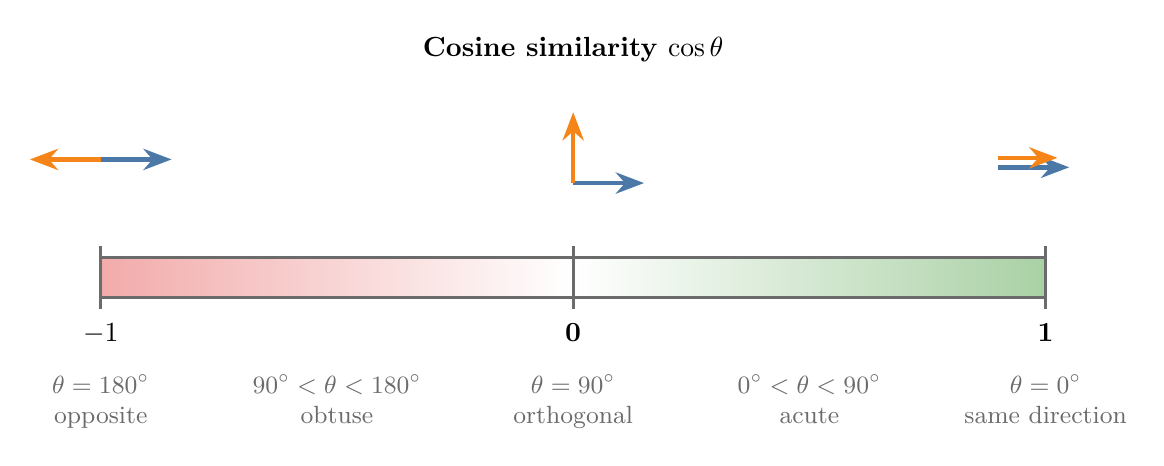
\begin{tikzpicture}
  \shade[left color=cred!50, right color=cgreen!50, middle color=white] (0,-0.25) rectangle (12,0.25);
  \draw[cgrey, line width=1pt] (0,-0.25) rectangle (12,0.25);
  \foreach \x/\l in {0/$-1$, 6/0, 12/1} { \draw[cgrey] (\x,-0.4) -- (\x,0.4); \node[below=0.45cm, font=\bfseries] at (\x,0) {\l}; }
  \node[font=\bfseries] at (6,2.9) {Cosine similarity $\cos\theta$};
  % little arrow pairs
  \begin{scope}[shift={(0,1.5)}]
    \draw[-{Stealth}, cblue, line width=1.6pt] (0,0) -- (0.9,0); \draw[-{Stealth}, corange, line width=1.6pt] (0,0) -- (-0.9,0);
  \end{scope}
  \begin{scope}[shift={(6,1.2)}]
    \draw[-{Stealth}, cblue, line width=1.6pt] (0,0) -- (0.9,0); \draw[-{Stealth}, corange, line width=1.6pt] (0,0) -- (0,0.9);
  \end{scope}
  \begin{scope}[shift={(11.4,1.4)}]
    \draw[-{Stealth}, cblue, line width=1.6pt] (0,0) -- (0.9,0); \draw[-{Stealth}, corange, line width=1.6pt] (0,0.12) -- (0.75,0.12);
  \end{scope}
  \node[note, below=1.1cm] at (0,0) {$\theta = 180^\circ$\\ opposite};
  \node[note, below=1.1cm] at (3,0) {$90^\circ < \theta < 180^\circ$\\ obtuse};
  \node[note, below=1.1cm] at (6,0) {$\theta = 90^\circ$\\ orthogonal};
  \node[note, below=1.1cm] at (9,0) {$0^\circ < \theta < 90^\circ$\\ acute};
  \node[note, below=1.1cm] at (12,0) {$\theta = 0^\circ$\\ same direction};
\end{tikzpicture}
\end{document}
